\documentclass[a4paper,14pt]{extarticle}

\usepackage{fontspec}
\usepackage{polyglossia}
\setmainlanguage{russian}
\setotherlanguage{english}

\setmainfont{Times New Roman}
\newfontfamily\cyrillicfont{Times New Roman}
\newfontfamily\cyrillicfonttt{Courier New}

\usepackage{graphicx}
\usepackage{geometry}
\usepackage{float}
\usepackage{amsmath}
\usepackage{amssymb}
\usepackage{setspace}
\usepackage{indentfirst}
\usepackage{listings}
\usepackage{xcolor}
\lstset{
    language=Python,
    basicstyle=\ttfamily\small,
    keywordstyle=\color{blue},
    commentstyle=\color{gray},
    stringstyle=\color{red!60!black},
    showstringspaces=false,
    breaklines=true,
    breakatwhitespace=true,
    columns=fullflexible,
    frame=single,
    tabsize=4,
    keepspaces=true
}
\geometry{left=30mm,right=15mm,top=20mm,bottom=20mm}
\setlength{\parindent}{1.25cm}
\onehalfspacing

\begin{document}

% ТИТУЛЬНЫЙ ЛИСТ

\begin{center}

\textbf{МИНИСТЕРСТВО НАУКИ И ВЫСШЕГО ОБРАЗОВАНИЯ\\
РОССИЙСКОЙ ФЕДЕРАЦИИ}

\vspace{0.6cm}

\textbf{ФЕДЕРАЛЬНОЕ ГОСУДАРСТВЕННОЕ БЮДЖЕТНОЕ\\
ОБРАЗОВАТЕЛЬНОЕ УЧРЕЖДЕНИЕ ВЫСШЕГО ОБРАЗОВАНИЯ\\
«БЕЛГОРОДСКИЙ ГОСУДАРСТВЕННЫЙ ТЕХНОЛОГИЧЕСКИЙ\\
УНИВЕРСИТЕТ им. В. Г. Шухова»\\
(БГТУ им. В. Г. Шухова)}


\vspace{0.6cm}


\includegraphics[width=0.22\textwidth]{logo.jpg}

\vspace{0.6cm}

Кафедра программного обеспечения вычислительной\\
техники и автоматизированных систем

\vspace{1.5cm}

\textbf{Лабораторная работа № 2}\\
по дисциплине: «Исследование операций»\\
на тему «Симплекс-метод в чистом виде»

\vspace{2cm}

\begin{flushright}
Выполнил: ст. группы ПВ-242\\
Кладченко Никита Сергеевич

\vspace{0.8cm}

Проверил:\\
Вирченко Юрий Петрович
\end{flushright}

\vfill

Белгород, 2026

\end{center}

\newpage

Цель работы: изучение симплекс-метода для решения задачи
линейного программирования с использованием симплекс-таблиц,
получение навыков кодирования изученного алгоритма, отладки и
тестирования соответствующих программ.

Задание:

1. Выяснить: какой вид должна иметь задача ЛП, чтобы можно было
применять симплекс-метод в чистом виде, а также как составляется
первая симплекс-таблица?

2. Изучить алгоритм перехода от одной симплекс-таблицы к другой
при решении задачи симплекс-методом.

3. Запрограммировать и отладить изученный алгоритм. В рамках
подготовки тестовых данных решить вручную одну из следующих
ниже задач.

Вариант 8:

\vspace{1cm}

\[
z = x_1 + 3x_2 - 5x_4 \rightarrow \max;
\]

\[
\left\{
\begin{aligned}
3x_1 + 4x_2 + x_3 + 2x_4 &= 27,\\
-4x_1 + 5x_2 - 3x_4 + x_5 &= 32,\\
5x_1 - 2x_2 + 8x_4 + x_6 &= 24,
\end{aligned}
\right.
\]

\[
x_i \geq 0 \quad (i=\overline{1,6}).
\]

\vspace{0.5cm}
\newpage
\textbf{Ход работы}

\textbf{Задание 1.} Выяснить: какой вид должна иметь задача ЛП, чтобы можно было
применять симплекс-метод в чистом виде, а также как составляется
первая симплекс-таблица?

Чтобы можно было применять симплекс-метод в чистом виде (прямой симплекс-метод), задача линейного программирования должна быть приведена к канонической форме, причём система ограничений должна находиться в допустимом базисном виде.

Каноническая форма задачи:

\begin{itemize}
\item Целевая функция подлежит максимизации:
\end{itemize}

\[
z=c_1 x_1+c_2 x_2+\cdots+c_n x_n\rightarrow\max
\]

\begin{itemize}
\item Все ограничения являются уравнениями:
\end{itemize}

\[
\left\{
\begin{aligned}
a_{11}x_1+\cdots+a_{1n}x_n&=b_1\\
\cdots \\
a_{m1}x_1+\cdots+a_{mn}x_n&=b_m
\end{aligned}
\right.
\]

\begin{itemize}
\item Все переменные неотрицательны:
\end{itemize}

\[
x_i\geq0,\; i=1,\ldots,n
\]

Допустимый базисный вид системы ограничений:

Система имеет допустимый базисный вид, если среди столбцов коэффициентов есть $m$ различных единичных столбцов, а правые части $b_i\geq0$. Переменные, соответствующие единичным столбцам, — базисные, остальные — свободные.

После приведения системы к базисному виду и подстановки базисных переменных в целевую функцию получаем:

\[
z=\gamma_0+\gamma_{r+1}x_{r+1}+\cdots+\gamma_n x_n,
\]

где $\gamma_0$ — значение целевой функции на текущем опорном решении.

\vspace{0.5cm}

Первая симплекс-таблица строится следующим образом:

\begin{center}
\begin{tabular}{|c|c|c|c|c|c|c|c|}
\hline
Базис & $b$ & $x_1$ & $x_2$ & $x_3$ & $x_4$ & $x_5$ & $x_6$ \\
\hline
$x_1$ & $b_1'$ & 1 & 0 & $\ldots$ & $\ldots$ & $\ldots$ & $\ldots$ \\
\hline
$\cdot$ & $\cdot$ & $\cdot$ & $\cdot$ & $\cdot$ & $\cdot$ & $\cdot$ & $\cdot$ \\
\hline
$\cdot$ & $\cdot$ & $\cdot$ & $\cdot$ & $\cdot$ & $\cdot$ & $\cdot$ & $\cdot$ \\
\hline
$\cdot$ & $\cdot$ & $\cdot$ & $\cdot$ & $\cdot$ & $\cdot$ & $\cdot$ & $\cdot$ \\
\hline
$x_m$ & $b_m'$ & 0 & $\ldots$ &  & 1 &  &  \\
\hline
$z$ & $\gamma_0$ & 0 & $-\gamma_2$ & $\ldots$ & $-\gamma_n$ &  &  \\
\hline
\end{tabular}
\end{center}

\textbf{Задание 2.} Изучить алгоритм перехода от одной симплекс-таблицы к другой
при решении задачи симплекс-методом.

Переход к новой симплекс-таблице соответствует замене одного опорного решения другим, на котором значение целевой функции не меньше предыдущего (для задачи на максимум). Ниже приведён пошаговый алгоритм симплекс-метода в чистом виде.

1. Проверка оптимальности текущего решения.

Просматриваем последнюю ($z$) строку таблицы (исключая столбец свободных членов). Если среди коэффициентов при переменных нет отрицательных, то текущее базисное решение является оптимальным. Процесс останавливается, ответ читается из последней таблицы.

Если есть отрицательные коэффициенты, решение можно улучшить — переходим к следующему шагу.

2. Выбор разрешающего столбца.

Среди отрицательных коэффициентов $z$-строки выбирается один. Рекомендуется выбирать наибольший по модулю отрицательный коэффициент (это соответствует переменной, увеличение которой сильнее всего повышает целевую функцию). Столбец, соответствующий этому коэффициенту, называется разрешающим.

3. Проверка на неограниченность целевой функции.

В разрешающем столбце (кроме $z$-строки) ищем положительные элементы.

• Если положительных элементов нет, то целевая функция неограничена на допустимом множестве. Задача не имеет конечного решения, алгоритм прекращает работу.

• Если положительные элементы есть — переходим к следующему пункту.

4. Выбор разрешающей строки (исключаемая переменная).

Для каждой строки $i$, в которой элемент разрешающего столбца

\[
a_{i,\text{разр}}>0
\]

вычисляется симплекс-отношение:

\[
\theta_i=\frac{b_i}{a_{i,\text{разр}}},
\]

где $b_i$ — свободный член в $i$-й строке. Выбирается строка с минимальным $\theta_i$. Переменная, стоящая в первом столбце этой строки, выводится из базиса.

5. Определение разрешающего элемента.

Элемент на пересечении разрешающей строки и разрешающего столбца называется разрешающим (генеральным) элементом $a_{pq}$.

6. Построение новой симплекс-таблицы (пересчёт).

• В первом столбце заменяем название базисной переменной на вводимую.

• Разрешающую строку делим на разрешающий элемент $a_{pq}$.

• Для каждой другой строки (включая $z$-строку) выполняем преобразование:

\[
\text{нов.эл.}_i=\text{ст.эл.}_i-a_{i,p}\cdot\text{нов.эл.}_p
\]

• В результате в разрешающем столбце новой таблицы должен получиться единичный вектор.

7. Возврат к шагу 1.

При выборе разрешающего столбца и строки возможны неоднозначности (несколько одинаковых минимальных симплекс-отношений или несколько максимальных по модулю отрицательных коэффициентов в $z$-строке). Для предотвращения зацикливания рекомендуется использовать правило Бланда (выбирать переменную с наименьшим индексом).

Критерии останова алгоритма:

• Успешное завершение: все коэффициенты в $z$-строке неотрицательны. В столбце свободных членов находятся значения базисных переменных оптимального решения, а в первой клетке $z$-строки — максимальное значение целевой функции.

• Неограниченность: в выбранном разрешающем столбце отсутствуют положительные элементы (шаг 3).

\textbf{Задание 3.} Запрограммировать и отладить изученный алгоритм. В рамках
подготовки тестовых данных решить вручную одну из следующих
ниже задач.

Исходная задача:

\[
z=x_1+3x_2-5x_4\rightarrow\max;
\]

\[
\left\{
\begin{aligned}
3x_1+4x_2+x_3+2x_4&=27,\\
-4x_1+5x_2-3x_4+x_5&=32,\\
5x_1-2x_2+8x_4+x_6&=24,
\end{aligned}
\right.
\]

\[
x_i\geq0 \quad (i=\overline{1,6})
\]

Приведём целевую функцию к виду, удобному для симплекс-таблицы:

\[
z-x_1-3x_2+5x_4=0.
\]

Начальный базис:

Единичные столбцы имеют переменные $x_3,x_5,x_6$, значит базис:

\[
x_3=27,x_5=32,x_6=24,
\]

\[
x_1=x_2=x_4=0,z=0.
\]

Первая симплекс-таблица:

\begin{center}
\begin{tabular}{|c|c|c|c|c|c|c|c|}
\hline
Базис & $b$ & $x_1$ & $x_2$ & $x_3$ & $x_4$ & $x_5$ & $x_6$ \\
\hline
$x_3$ & 27 & 3 & 4 & 1 & 2 & 0 & 0 \\
\hline
$x_5$ & 32 & -4 & 5 & 0 & -3 & 1 & 0 \\
\hline
$x_6$ & 24 & 5 & -2 & 0 & 8 & 0 & 1 \\
\hline
$z$ & 0 & -1 & -3 & 0 & 5 & 0 & 0 \\
\hline
\end{tabular}
\end{center}

\textbf{Итерация 1}

В $z$-строке есть отрицательные коэффициенты: -1, -3

Берём максимальный по модулю: -3 → столбец $x_2$

Проверка столбца $x_2$:

\[
\theta_1=\frac{27}{4}=6.75
\]

\[
\theta_2=\frac{32}{5}=6.4
\]

Минимум: 6.4 → строка $x_5$

Разрешающий элемент: 5.

Нормализация строки $x_5$:

\[
x_2=(6.4,-0.8,1,0,-0.6,0.2,0)
\]

Пересчёт таблицы методом Гаусса–Жордана:

Строка $x_3$:

\[
b'=27-4\cdot6.4=1.4
\]

\[
x_1'=3-4\cdot(-0.8)=6.2
\]

\[
x_2'=4-4\cdot1=0
\]

\[
x_3'=1-4\cdot0=1
\]

\[
x_4'=2-4\cdot(-0.6)=4.4
\]

\[
x_5'=0-4\cdot0.2=-0.8
\]

\[
x_6'=0-4\cdot0=0
\]

Строка $x_6$:

\[
b'=24-(-2)\cdot6.4=36.8
\]

\[
x_1'=5-(-2)\cdot(-0.8)=3.4
\]

\[
x_2'=-2-(-2)\cdot1=0
\]

\[
x_3'=0-(-2)\cdot0=0
\]

\[
x_4'=8-(-2)\cdot(-0.6)=6.8
\]

\[
x_5'=0-(-2)\cdot0.2=0.4
\]

\[
x_6'=1-(-2)\cdot0=1
\]

$z$-строка:

\[
b'=0-(-3)\cdot6.4=19.2
\]

\[
x_1'=-1-(-3)\cdot(-0.8)=-3.4
\]

\[
x_2'=-3-(-3)\cdot1=0
\]

\[
x_3'=0-(-3)\cdot0=0
\]

\[
x_4'=5-(-3)\cdot(-0.6)=3.2
\]

\[
x_5'=0-(-3)\cdot0.2=0.6
\]

\[
x_6'=0-(-3)\cdot0=0
\]

Вторая таблица:

\begin{center}
\begin{tabular}{|c|c|c|c|c|c|c|c|}
\hline
Базис & $b$ & $x_1$ & $x_2$ & $x_3$ & $x_4$ & $x_5$ & $x_6$ \\
\hline
$x_3$ & 1.4 & 6.2 & 0 & 1 & 4.4 & -0.8 & 0 \\
\hline
$x_2$ & 6.4 & -0.8 & 1 & 0 & -0.6 & 0.2 & 0 \\
\hline
$x_6$ & 36.8 & 3.4 & 0 & 0 & 6.8 & 0.4 & 1 \\
\hline
$z$ & 19.2 & -3.4 & 0 & 0 & 3.2 & 0.6 & 0 \\
\hline
\end{tabular}
\end{center}

\textbf{Итерация 2}

В $z$-строке есть отрицательный: -3.4 → $x_1$

Проверка:

\[
\theta_1=\frac{1.4}{6.2}\approx0.226
\]

\[
\theta_3=\frac{36.8}{3.4}\approx10.82
\]

Выбираем $x_3$.

Нормализация $x_3$:

\[
x_1=(0.226,1,0,0.161,0.709,-0.129,0)
\]

Результат:

\[
x_1\approx0.226,x_2\approx6.4,x_3=0,x_4=0,x_5=0,x_6\approx36.8
\]

\[
z_{\max}\approx19.2
\]

Все коэффициенты в $z \geq 0$ → оптимум достигнут.

Проверка подстановкой в целевую функцию: \[0.226 + 3 \cdot 6.4 – 5 \cdot 0 = 19.2\] — совпадает. Проверка подстановкой в исходные уравнения также подтверждает допустимость решения.

\vspace{1cm}

Код программы:

\begin{lstlisting}
import numpy as np

EPS = 1e-9


def build_tableau(a_matrix, b_vector, c_vector):
    a_matrix = np.array(a_matrix, dtype=float)
    b_vector = np.array(b_vector, dtype=float)
    c_vector = np.array(c_vector, dtype=float)

    m, n = a_matrix.shape

    tableau = np.zeros((m + 1, n + 1), dtype=float)
    tableau[:m, 0] = b_vector
    tableau[:m, 1:] = a_matrix
    tableau[m, 1:] = -c_vector

    return tableau


def choose_pivot(tableau):
    rows = tableau.shape[0] - 1
    cols = tableau.shape[1] - 1

    z_row = tableau[rows, 1:]

    if np.all(z_row >= -EPS):
        return -1, -1

    pivot_col = np.argmin(z_row) + 1

    col = tableau[:rows, pivot_col]
    rhs = tableau[:rows, 0]

    valid = col > EPS
    if not np.any(valid):
        return None, None

    ratios = np.full(rows, np.inf)
    ratios[valid] = rhs[valid] / col[valid]

    pivot_row = np.argmin(ratios)
    return pivot_row, pivot_col


def pivot_transform(tableau, pivot_row, pivot_col):
    pivot_elem = tableau[pivot_row, pivot_col]
    tableau[pivot_row, :] /= pivot_elem

    for i in range(tableau.shape[0]):
        if i != pivot_row:
            factor = tableau[i, pivot_col]
            tableau[i, :] -= factor * tableau[pivot_row, :]


def print_tableau(tableau, basis, iteration):
    rows, cols = tableau.shape
    var_count = cols - 1

    print(f"\nИтерация {iteration}")
    print("-" * (12 * (var_count + 2)))

    header = f"{'Базис':>8}{'b':>10}"
    for j in range(1, var_count + 1):
        header += f"{('x' + str(j)):>10}"
    print(header)

    for i in range(rows):
        if i < rows - 1:
            row_name = f"x{basis[i]}"
        else:
            row_name = "z"

        line = f"{row_name:>8}"
        for j in range(cols):
            line += f"{tableau[i, j]:>10.4f}"
        print(line)

def simplex_solve(a_matrix, b_vector, c_vector, basis, verbose=True):
    tableau = build_tableau(a_matrix, b_vector, c_vector)
    basis = basis[:]

    iteration = 1

    while True:
        if verbose:
            print_tableau(tableau, basis, iteration)

        pivot_row, pivot_col = choose_pivot(tableau)

        if pivot_row == -1:
            solution = np.zeros(tableau.shape[1] - 1)
            for i in range(len(basis)):
                solution[basis[i] - 1] = tableau[i, 0]
            optimum = tableau[-1, 0]
            return "ok", solution, optimum, tableau

        if pivot_row is None:
            return "Целевая функция не ограничена", None, None, tableau

        pivot_transform(tableau, pivot_row, pivot_col)
        basis[pivot_row] = pivot_col

        iteration += 1


if __name__ == "__main__":
    # Вариант 8
    # z = x1 + 3x2 - 5x4 -> max
    # 3x1 + 4x2 + x3 + 2x4 = 27
    # -4x1 + 5x2 - 3x4 + x5 = 32
    # 5x1 - 2x2 + 8x4 + x6 = 24

    A = [
        [3, 4, 1, 2, 0, 0],
        [-4, 5, 0, -3, 1, 0],
        [5, -2, 0, 8, 0, 1]
    ]

    b = [27, 32, 24]
    c = [1, 3, 0, -5, 0, 0]

    # Начальный базис: x3, x5, x6
    basis = [3, 5, 6]

    status, solution, optimum, final_tableau = simplex_solve(A, b, c, basis, verbose=True)

    print("\n Статус:", status)
    if status == "ok":
        print("Оптимальный план x:", solution)
        print("Максимум z:", optimum)
\end{lstlisting}

\begin{figure}[H]
\centering
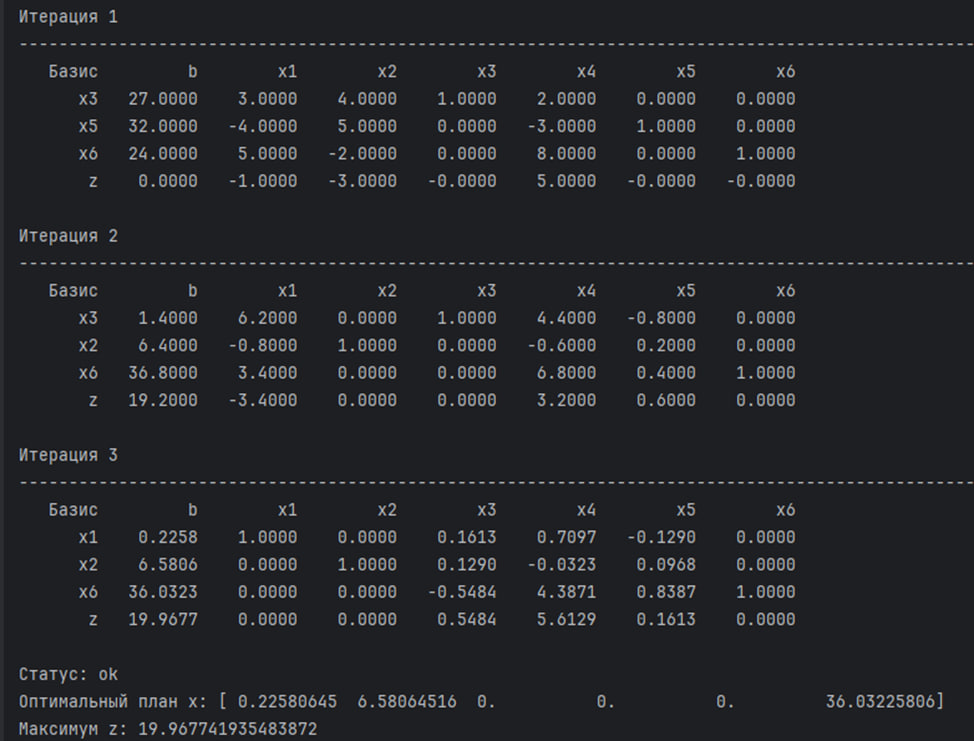
\includegraphics[width=0.9\textwidth]{result.jpg}
\caption{Результат работы программы}
\end{figure}

\begin{figure}[H]
\centering

\includegraphics[width=0.9\textwidth]{main.png}
\caption{Блок-схема функции main}
\end{figure}

\begin{figure}[H]
\centering

\includegraphics[width=0.9\textwidth]{build_tableau.png}
\caption{Блок-схема функции build\_tableau}
\end{figure}

\begin{figure}[H]
\centering

\includegraphics[width=0.7\textwidth]{choose_pivot.png}
\caption{Блок-схема функции choose\_pivot}
\end{figure}

\begin{figure}[H]
\centering

\includegraphics[width=0.9\textwidth]{pivot_transform.png}
\caption{Блок-схема функции pivot\_transform}
\end{figure}

\begin{figure}[H]
\centering

\includegraphics[width=0.9\textwidth]{print_tableau.png}
\caption{Блок-схема функции print\_tableau}
\end{figure}

\begin{figure}[H]
\centering

\includegraphics[width=0.9\textwidth]{ContPrint_tableau.png}
\caption{Продолжение блок-схемы функции print\_tableau}
\end{figure}

\begin{figure}[H]
\centering

\includegraphics[width=0.9\textwidth]{simplex_solve.png}
\caption{Блок-схема функции simplex\_solve}
\end{figure}

\begin{figure}[H]
\centering

\includegraphics[width=0.9\textwidth]{ContSimplex_solve.png}
\caption{Продолжение блок-схемы функции simplex\_solve}
\end{figure}
\textbf{Вывод:}
 в ходе работы был изучен прямой симплекс-метод решения задач линейного программирования в канонической форме и рассмотрен принцип построения первой симплекс-таблицы на основе допустимого базисного решения. Был разобран алгоритм перехода от одной симплекс-таблицы к другой: проверка оптимальности по строке целевой функции, выбор разрешающего столбца и строки, проверка на неограниченность. На основе изученного алгоритма была разработана и отлажена программа, реализующая основные этапы симплекс-метода: построение начальной таблицы, выбор разрешающего элемента, выполнение pivot-преобразований и формирование итогового решения. Для выбранного варианта задача была решена аналитически. Результат программы совпал с аналитическими расчётами: найден допустимый оптимальный план и значение целевой функции. Таким образом, поставленная цель работы достигнута: получены практические навыки реализации, отладки и тестирования симплекс-метода.

\end{document}